\begin{figure}[ht!]
\centering
  \subfloat[$SE^1_y$] {
    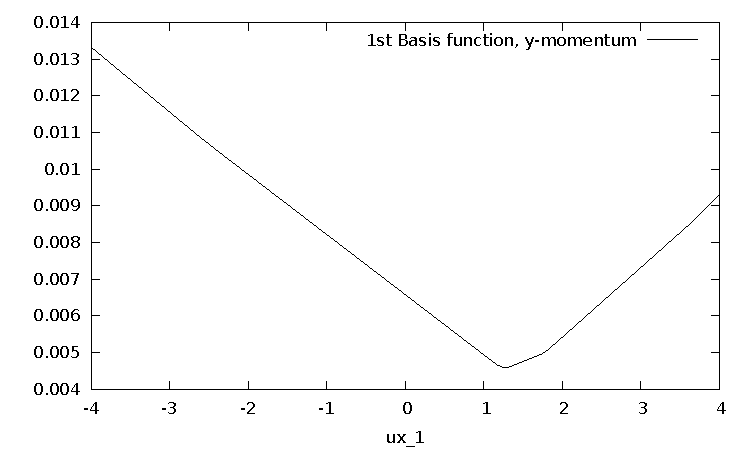
\includegraphics[scale=\zoomfactor]{{{ord2_varying_ux1_uy2_1/10.0_10.0_10.0_10.0_10.0_10.0_y_0.0_0.0_0.0_0.0_0.0_0.0_1.0_0.0_0.0_0.0_0.0f01}}}
  }
  \subfloat[$SE^2_y$] {
    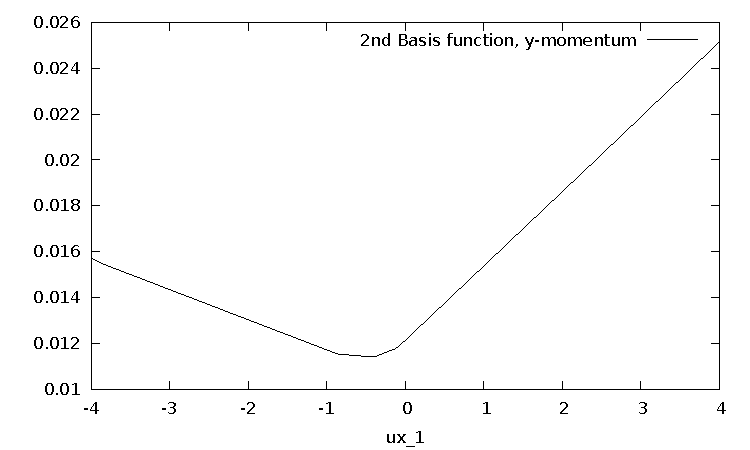
\includegraphics[scale=\zoomfactor]{{{ord2_varying_ux1_uy2_1/10.0_10.0_10.0_10.0_10.0_10.0_y_0.0_0.0_0.0_0.0_0.0_0.0_1.0_0.0_0.0_0.0_0.0f03}}}
  }
  \subfloat[$SE^3_y$] {
    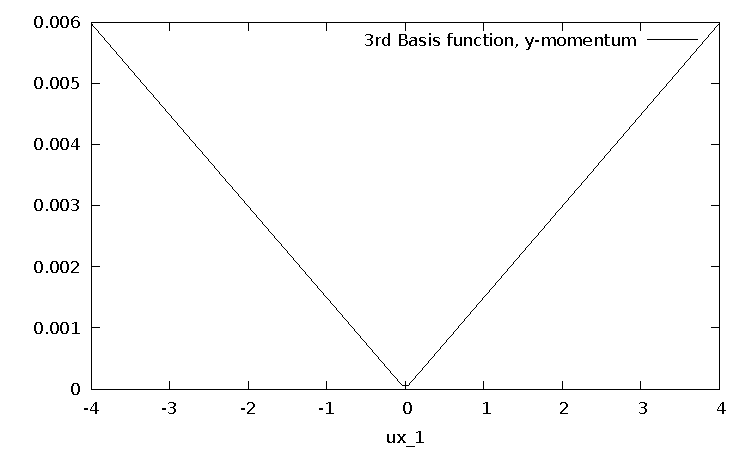
\includegraphics[scale=\zoomfactor]{{{ord2_varying_ux1_uy2_1/10.0_10.0_10.0_10.0_10.0_10.0_y_0.0_0.0_0.0_0.0_0.0_0.0_1.0_0.0_0.0_0.0_0.0f05}}}
  }
  \subfloat[$SE^4_y$] {
    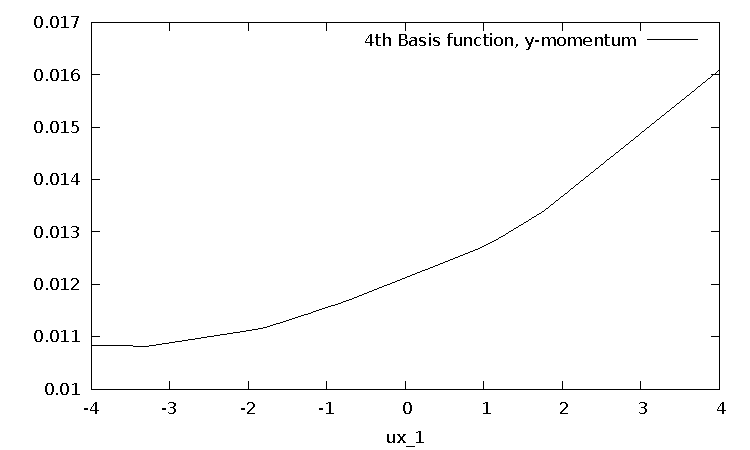
\includegraphics[scale=\zoomfactor]{{{ord2_varying_ux1_uy2_1/10.0_10.0_10.0_10.0_10.0_10.0_y_0.0_0.0_0.0_0.0_0.0_0.0_1.0_0.0_0.0_0.0_0.0f07}}}
  }
  \subfloat[$SE^5_y$] {
    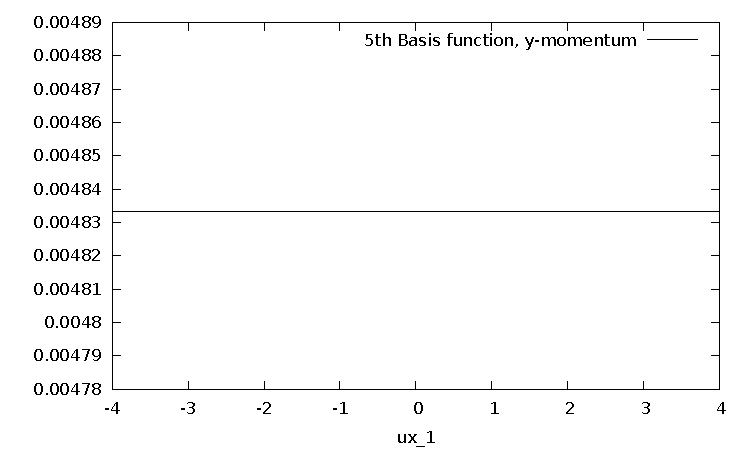
\includegraphics[scale=\zoomfactor]{{{ord2_varying_ux1_uy2_1/10.0_10.0_10.0_10.0_10.0_10.0_y_0.0_0.0_0.0_0.0_0.0_0.0_1.0_0.0_0.0_0.0_0.0f09}}}
  }
  \subfloat[$SE^6_y$] {
    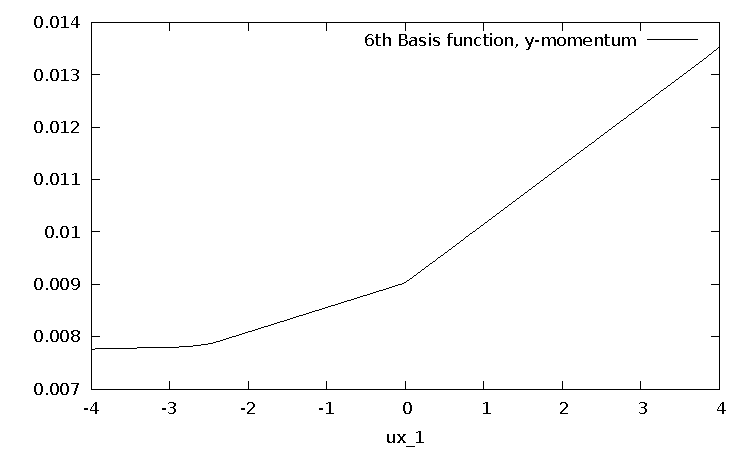
\includegraphics[scale=\zoomfactor]{{{ord2_varying_ux1_uy2_1/10.0_10.0_10.0_10.0_10.0_10.0_y_0.0_0.0_0.0_0.0_0.0_0.0_1.0_0.0_0.0_0.0_0.0f11}}}
  }
\caption{Error plots for $y$-momentums. All heights are 10, and all momentums except $u_{x,1}$ and $u_{y,2}$ are fixed to 0. The value $u_{y,2}$ is set to 1.}
\label{fig:ord2_varying_ux1_uy2_1__ycomponent}
\end{figure}

%%% Local Variables:
%%% TeX-master: "../results.tex"
%%% End:
